% !TEX root = ../IS.tex
\chapter{Machine Learning}
\section{Decision Trees}
The goal of a machine learning problem is, of course, to learn; given a task with a particular performance measure, the performance can be improved through some kind of training or experience. Often, this involves evaluating a general case for the task from a set of specific examples \cite{mitc97}. One of the more common machine learning techniques is the decision tree. It can approximate discrete-valued functions \cite{mitc97} and automatically classify data \cite{sega07}. Generally, decision trees focus on problems with attribute-value pairs; an attribute \textit{Temperature} may have the possible values \textit{Hot, Cold, Warm, Cool} \cite{mitc97}.\\

When creating a decision tree, one must begin with example data to analyze. This may be historical data, looking at the same type of results from previous years in order to predict current trends, or a self-contained set of data to be used on similar inputs. In order to form an effective tree, these data are split into two groups: a training set, and a testing set. The training set is used to create the tree, while the testing set is used to find the approximate error of the tree. It is important that these two sets are disjoint; the error of a tree cannot be accurately determined if it isn't analyzing new data in the testing phase.

\subsection{ID3 Algorithm}
The ID3 algorithm for decision trees, like most decision tree algorithms, uses a top-down greedy search \cite{mitc97}. The algorithm begins by evaluating the input data by individual attributes in the training set. For each attribute, the algorithm attempts to classify the entire data set using only that attribute. Whichever attribute was the most successful on its own becomes the root of the tree. Then, for each possible value of that root attribute, a descendant node is created and the training set is split accordingly. Then, for each descendant node and its respective subset of training data, the process is repeated.\\

To find the best attribute at each node of the tree, the ID3 algorithm uses the statistical property information gain. Information gain utilizes entropy, or the relative impurity of a data collection.
\begin{define}
  For a set of training data $S$ with $n$ different target values, Entropy(S)$\equiv\sum_{i=1}^n-p_i$log$_2p_i$, where $p_i$ is the proportion of S with a target value of $i$.
\end{define}
Entropy calculations define 0log(0) as 0. The logarithm can have any base value, but two is often used; a base of 2 conveys the expected encoding length in bits \cite{mitc97}. Assuming the base value is 2, an entropy value of 0 occurs when all data set elements have the same target value $i$, and a  set with a 50/50 split between two target values will have an entropy value of 1. Ideally, a decision tree classifies data into sets with low entropy, as this indicates an accurate tree structure.\\

In order to minimize entropy in the classified data, the information gain of each attribute is calculated. Information gain is defined as the expected reduction in entropy caused by splitting the training data by a particular attribute.
\begin{define}
  For an attribute $A$ and a set of training data $S$, the Information Gain(S, A)$\equiv$ Entropy(S) $-\sum_{v\in Values(A)}\frac{||S_v||}{||S||}$ Entropy$(S_v)$, where $Values(A)$ is the set of possible values for the attribute $A$, and $S_v$ is the subset of $S$ where $A$ has value $v$.
\end{define}
Each attribute $A$ for a given node is tested, with each of its possible values used in the summation. For these values, the entropy of each subset $S_v$ is calculated, then scaled by the size of $S_v$ compared to $S$.\\

\begin{figure}[H]
  \centering
  \begin{tabular}{| c | c | c |}
    Month & Tickets & Weekend \\ \hline
    3 & 25 & 0 \\ \hline
    8 & 45 & 1 \\ \hline
    8 & 25 & 0 \\ \hline
  \end{tabular}
  \caption{A sample data set with three attributes and three entries}
  \label{fig:ExampleEntropy}
\end{figure}

For example, consider the data set in Figure \ref{fig:ExampleEntropy}. The \textit{Month} attribute is the numeric value of the calendar month, \textit{Tickets} is the number of tickets sold to an event, and \textit{Weekend} is a Boolean value whether the event is on a weekend or not. Suppose that the target attribute of this set is \textit{Weekend}. The \textit{Weekend} attribute has two values represented in the set: 0 and 1. Of the data points in Figure \ref{fig:ExampleEntropy}, only one took place on a weekend. Thus, the $p_i$ for Weekend=True is $\frac{1}{3}$, which we round to $.33$. The $p_i$ for Weekend=False is therefore $\frac{2}{3}$ rounded to $.66$. Recall that the entropy formula is Entropy(S)$\equiv\sum_{i=1}^n-p_i$log$_2p_i$. Let $i=1$ be the attribute Weekend=True and $i=2$ be the attribute Weekend=False. The entropy for the target attribute \textit{Weekend} is therefore the sum $-.66$log$_2(0.66) + -.33$log$_2(.33)$, or approximately 0.9235. For this specific set, all attributes have two possible values, and will thus have a $\frac{1}{3}$ and $\frac{2}{3}$ split. In this example, the entropy will be the same for any target attribute.\\

To reduce this entropy, the ID3 algorithm finds the information gain for the two non-target attributes: \textit{Month} and \textit{Tickets}. Beginning with \textit{Month}, the information gain is $0.9235 - \frac{1}{3}$(Entropy(v=3)) $+ \frac{2}{3}$(Entropy(v=8)). At \textit{Month} 3, the entropy of the set is 0, as it contains a single element. The entropy of the subset at \textit{Month}=8 is 1, as the set has a 50/50 split along the target \textit{Weekend} attribute. Thus, the information gain for \textit{Month} is $0.9235 - \frac{2}{3}$, or 0.2568. Separating the data set along the \textit{Month} attribute does help in classifying the events by weekend, but the August events are now split 50/50.\\

The \textit{Tickets} attribute has an information gain of $0.9235 - \frac{2}{3}$(Entropy(v=25)) $+ \frac{1}{3}$(Entropy(v=45)). Since all elements in the subset of $S$ where \textit{Tickets}=25 have a target values of 0, the entropy is 0. The same is true of the subset where \textit{Tickets}=45. Thus, the information gain from this attribute is 0.9235. This does not indicate that no information was gained, this indicates that all entropy was removed from the set. All subsets are homogeneous when separating subsets by \textit{Tickets}.

Once the maximum information gain for a set has been determined, the ID3 algorithm uses the resulting subsets and recursively creates new subtrees for the subsets. This process continues until the entropy for the entire tree is 0. Once a tree has been created with the algorithm, it is simple to classify new data. Starting at the root of the tree, each target attribute is tested recursively, moving from one node to another down the tree \cite{sega07}.\\

\lstset{language=pseudocode, label=lst:ID3, caption={The ID3 Decision Tree algorithm \cite{mitc97}.}}
\begin{lstlisting}
Procedure ID3(TrainingSet S, TargetAttribute t, AttributeSet A)
create node Root
TestEntropy = True, TestAttributeValue = S[0]
for(i in S)  //Check whether the TrainingSet is uniform on t
  if(TargetAttribute[i]!=TestAttributeValue) TestEntropy=False
  //One of the elements has a different value for t
  end if
end for
if(TestEntropy is True) return root with label value of t
//This is a single-node tree; all elements in S have the same t value
else if(A is EmptySet) return Root with mode(t)
//There are no more attributes to check, return most common t value
else
//Determine optimal split for S
  OptimalInformationGain = 0
  for(attr in A)
    InformationGain = Entropy(S)
    EntropySum = 0
    for(val in attr)
      S_v = {S:Value(attribute)=val} //S_v contains the elements of S which have val for attr
      EntropySum = EntropySum + size(S_v)/size(S) * Entropy(S_v)  //Add entropy for each possible val for attr
    end for
    InformationGain = InformationGain - EntropySum
    //This is the information gain from splitting S on attr
    if(InformationGain > OptimalInformationGain)
      OptimalInformationGain = InformationGain
      //The maximum InformationGain value is stored
    end if
  end for
  //The optimal information gain has been found on attr
  Root.Label = attr
  for(val in attr)
    create Branch(val_i)
    NewTrainingData = {s in S:Value(attr)=val_i}
    if(NewTrainingData is EmptySet)
      create Leaf with mode(t) on S
    else
      add ID3(NewTrainingData, t, A-attr) as subtree
    end if
  end for
end if
return Root
end Procedure
\end{lstlisting}

In line 2 of the algorithm in Listing \ref{lst:ID3}, the root of the tree (or subtree) is created. The first base case to test is whether or not the TargetAttribute $t$ has the same value for every element in the TrainingSet $S$. This base case refers to a set $S$ with an entropy of 0, that requires no further classification, and begins at line 5. The second base case, starting on line 15, occurs when no non-target attributes remain in $A$. Without attributes, there is no way to further classify $S$, and the most common value for $t$ is used as the label for this node. This leaves the recursive case. The first step is to find the optimal information gain, and thus the next attribute used to split $S$. The loop at line 21 checks each attribute in $A$ for the largest reduction in entropy, and the attribute that created this reduction is saved as the label for the Root node on line 38. Line 39's loop prepares the data to be analyzed by the next levels of the decision tree. First, a new branch is created linking Root and the to-be-created subtree, with each branch labeled with a possible value of the attribute used in the split. Training data is split along this same value. If one of the new training data splits has no elements, a leaf node is labeled with the most common value of $t$ in $S$. This step is done to accommodate future data sets; while the training set may not have had any examples with that attribute value, other sets might and thus the tree assumes the most common value is correct. All other splits of $S$ are recursively passed to ID3() in line 45, along with $t$ and the AttributeSet $A$ (sans the attribute just used).\\

Suppose someone wanted to use the data set in Figure \ref{fig:ExampleEntropy} to predict ticket sales. We have the TargetAttribute \textit{Tickets}, an AttributeSet \{\textit{Month, Weekend}\}, and a TrainingSet = \{(3, 25, 0), (8, 45, 1), (8, 25, 0)\}. After creating a root node, we first check if all values of the TargetAttribute \textit{Tickets} are the same in the data set. This is not the case (two instances of 25 tickets sold, one instance of 45 tickets sold), so we continue through the algorithm. The second step is to check if AttributeSet is the empty set; this also is not the case. Thus, we enter the meat of the algorithm. We choose an attribute from AttributeSet and find the information gain of that attribute. Recall that the information gain of an attribute $A$ and set of examples $S$ is equal to Entropy$(S)-\sum_{v\in Values(A)}\frac{||S_v||}{||S||}$ Entropy$(S_v)$. As established previously, the entropy of our TrainingSet is approximately $0.9235$. With three entries, $||S||=3$. To start, let $A$ be the attribute \textit{Month}, which has possible values 3 and 8. For $v=3$, the subset $S_v$ has one entry, so $||S_v||=1$. In a set with only one entry, the entropy will necessarily be 0. For $v=8$, $S_v$ has two entries and $||S_v||=2$. The two August entries have different values for \textit{Tickets}, so the proportion $p_i$ will be $\frac{1}{2}$. Thus, the entropy of $S_v$ for $v=8$ will be $-.5 $log$_2(.5)$, which is $.5$. Thus, the information gain for attribute \textit{Month} is:
\begin{align*}
  .9235 - [(\frac{1}{3}*0) + (\frac{2}{3}*.5]\\
  .9235 - [0 + \frac{1}{3}]\\
  .5902
\end{align*}

Next, we repeat this formula for attribute \textit{Weekend}. This attribute also has two possible values, 1 and 0. For $v=1$, there is only one entry; $||S_v||$ will again be 1 and entropy will again be zero. For $v=0$, there are two entries, so $||S_v||=2$. Both of these entries have the same value for the target attribute \textit{Tickets}, so the entropy on $S_v$ for $v=0$ is also 0. Thus, the information gain for attribute \textit{Weekend} is:
\begin{align*}
  .9235 - [(\frac{1}{3}*0) + (\frac{2}{3}*0)]\\
  .9235 - [0 + 0]\\
  .9235
\end{align*}
We find that the \textit{Weekend} attribute has a higher information gain than the \textit{Month} attribute. So, the next step in the algorithm is to label the root node with \textit{Weekend}. 

\begin{figure}[H]
  \centering
  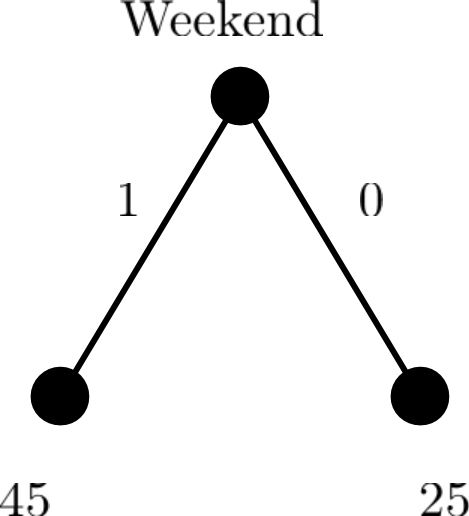
\includegraphics[width=4cm]{figures/ID3Example.png}
  \caption{A decision tree made with the ID3 algorithm, based on the training set in Figure \ref{fig:ExampleEntropy} with TargetAttribute \textit{Tickets}}
  \label{fig:ID3Example}
\end{figure}
Then, for the two possible values of \textit{Weekend}, the algorithm creates a new branch for that value. For the branch where $v=1$, the ID3 algorithm is called with TargetAttribute \textit{Tickets}, AttributeSet \{\textit{Month}\}, and TrainingSet = \{(8, 45, 1)\}. In this recursive call, the TargetAttribute \textit{Tickets} is uniform. Thus, the recursive call returns a node labeled with the value of \textit{Tickets}, 45. For the branch where $v=0$, the ID3 algorithm is called with TargetAttribute \textit{Tickets}, AttributeSet \{\textit{Month}\}, and TrainingSet = \{(3, 25, 0), (8, 25, 0)\}. Again, the TargetAttribute \textit{Tickets} is uniform, so a node labeled with the value of \textit{Tickets}, 25, is returned. Thus, the ID3 algorithm returns the tree in Figure \ref{fig:ID3Example}.\\

Once the tree is generated by the ID3 algorithm, classifying new data is simple. Suppose a new data set point is used, with \textit{Weekend} equal to True (or 1) and \textit{Month} equal to 5. Using the example in Figure \ref{fig:ID3Example}, this event would be predicted to have 45 tickets sold.\\

\subsection{Special Cases}
While the data in Figure \ref{fig:ExampleEntropy} use numeric data, the small sample set allows the ID3 algorithm to treat them as discrete values. However, decision trees must also be able to classify along continuous-valued attributes.
\begin{figure}[H]
  \centering
  \begin{tabular}{| c | c |}
    Temperature & Played Tennis \\ \hline
    40 & No \\ \hline
    48 & No \\ \hline
    60 & Yes \\ \hline
    72 & Yes \\ \hline
    80 & Yes \\ \hline
    90 & No \\ \hline
  \end{tabular}
  \caption{A sample data set containing the temperature in degrees Fahrenheit and whether or not tennis was played \cite{mitc97}.}
  \label{fig:rangedValue}
\end{figure}

\begin{exmp}
  Take for example the data set in Figure \ref{fig:rangedValue}. This data set is being analyzed to determine which temperatures are ideal for playing tennis. For six days, the temperature in degrees Fahrenheit and whether people played tennis was recorded.\\
\end{exmp}

Since only six temperatures were recorded, this training set cannot use these findings as discrete values. If it was classified discretely, then any temperature not explicitly in the training set (68 degrees, for instance) would not be accurately classified. Thus, the temperature must be treated as a continuous-valued attribute.\\

To deal with a continuous-valued attribute $A$, a new Boolean attribute $A_c$ is created where $A_c$ is true if $A<c$ and false otherwise \cite{mitc97}. For the dataset in Figure \ref{fig:rangedValue}, $c$ should be set to a value where the target attribute (in this example, whether people played tennis) changes. Thus, for this example, the thresholds between whether people do play tennis or when they don't happens between 48 and 60 degrees, and between 80 and 90 degrees. The simplest method is to take the average of the two temperatures, so $A_{c1}=\frac{48+60}{2}=54$ and $A_{c2}=\frac{80+90}{2}=85$. Therefore, based on the training data, a decision tree classifying tennis by outdoor temperature would predict ``No'' when temperature is below 54 degrees or above 85 degrees, and ``Yes'' when the temperature is between 54 and 85 degrees.\\

Another hurdle with decision trees comes when a data set has missing values for particular attributes $A$. There are two strategies for dealing with these cases: assign the element the most common value of $A$ in the rest of the data set, or assign probabilities for each possible value of $A$ \cite{mitc97}. 

\subsection{Optimizing the Tree}
Decision trees are susceptible to overfitting, where decisions at each node are too closely tied to the training set. Overfitting is caused by an algorithm creating superfluous branches that slightly decrease entropy for the set, but are in fact arbitrary decisions \cite{sega07}. For example, a decision tree could be created to classify students to their fields of study. An overfitted tree might contain choice nodes checking the names of the students. The tree is able to reach 0 entropy on the training set by classifying all students named ``John Smith'' as an English major and all students named ``Jane Doe'' as a Chemistry major, but this tree would not correctly classify a music major named John Smith.\\

There are two common methods to prevent overfitting. The first method is to require a minimum reduction in entropy at each split. Once the minimum is not reached, the tree stops creating additional branches. While commonly used, this method is insufficient in cases where early splits do not reduce entropy, but later splits greatly reduce the entropy of the set \cite{sega07}. The second method is to build the tree, then prune any extraneous nodes. Working from the bottom-up, the tree examines two leaf nodes with the same parent and determines whether merging these nodes does not increase entropy more than a specified threshold. If the nodes pass this test, they are combined and their parent becomes a new leaf node.\\

\section{Conclusion}
Decision trees are a useful tool to evaluate a data set, determine correlations between attributes and a target value, and create a tree to classify new data on these target values. The ID3 algorithm, one of the more common methods of creating a decision tree, examines each possible split of attributes to find the greatest reduction in the dataset's entropy, then creates a new branch on the tree using the attribute split. This process continues until all attributes are used or all data points have the same target value. The tree can be optimized by requiring a split in the tree to have some level of reduction in entropy. Once a tree is created, new data is classified by starting at the top of the decision tree, then following the branches until a target value is given.